\chapter{Ultrasonido}
%\stepcounter{chapter}

\section{Objetivo}
Implementar un circuito capaz de hacer mediciones de distancia con un sensor ultrasonico HC-SR04 (diseñado para ser usado en Arduino) sin el uso de ningún tipo de logica programable. La función de dicho sensor es la de medir distancias de entre 5cm y 4m. Sin embargo no es posible medir de manera directa con el mismo, se debe recurrir a una medición indirecta. El sensor ultrasonico disparara una serie de pulsos no audibles a 40Khz. Luego, el mismo recibira una señal de \emph{ECHO} producto del rebote entre la señal de salida y el objeto del cual reboto. 
\begin{center}
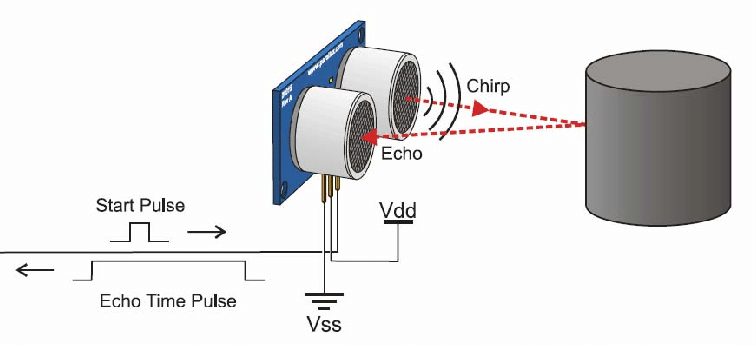
\includegraphics[scale=0.5]{../8-UltraSound/HC-SR04 diagram.png}
\end{center}
\section{Análisis}
Para poder empezar con el proceso de diseño se analizaron todas las etapas por las que deberian viajar las señales con el fin de realizar lo pedido.
\begin{center}
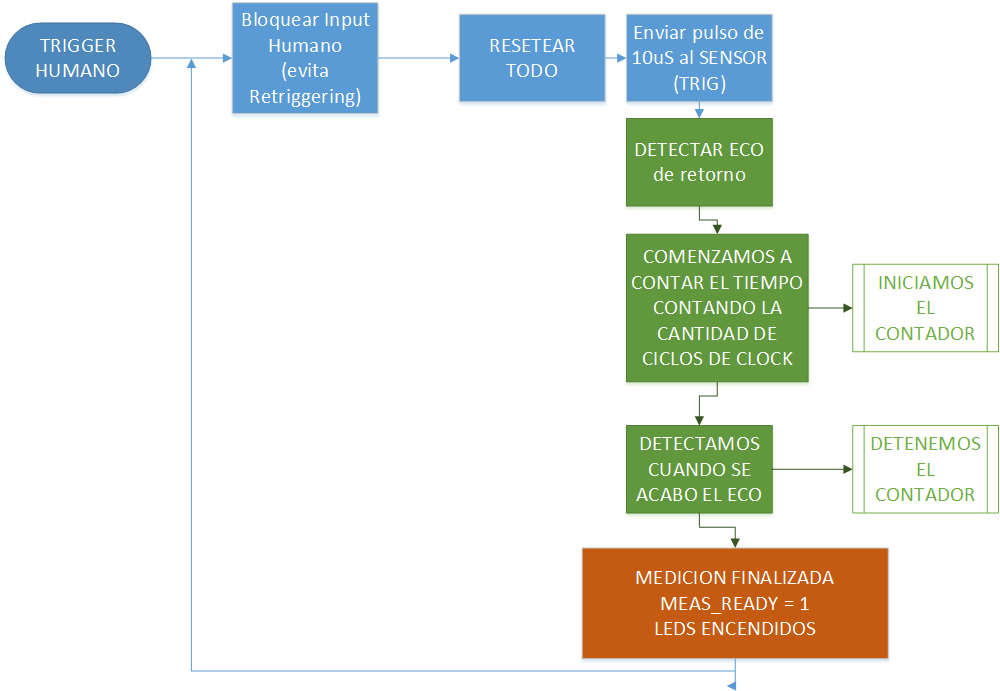
\includegraphics[scale=0.5]{../8-UltraSound/Diagrama-de-Flujo.png}
\end{center}
El diseño comienza por la construcción de un sistema de trigger que permita los procesos que desencadenaran los demás bloques del circuito.
Para dicho sistema se podria haber optado por la implementación de un pulsador tradicional. Sin embargo eso trae ciertos inconvenietes de implementación. Estos percances tienen su raiz en la naturaleza de funcionamiento del multivibrador \emph{LM555}.
Además en secciones posteriores se justificara la no implementación de la etapa de bloqueo.
\section{Generador de puslos con LM555 Monoestable}
El objetivo del \emph{LM555} es la de generar un pulso de mayor o igual a 10 $\mu S$ con el fin de poder triggerear el HC-SR04 y que este emita un tren de pulsos a frecuencias no audibles para evitar interferencias.

\begin{center}
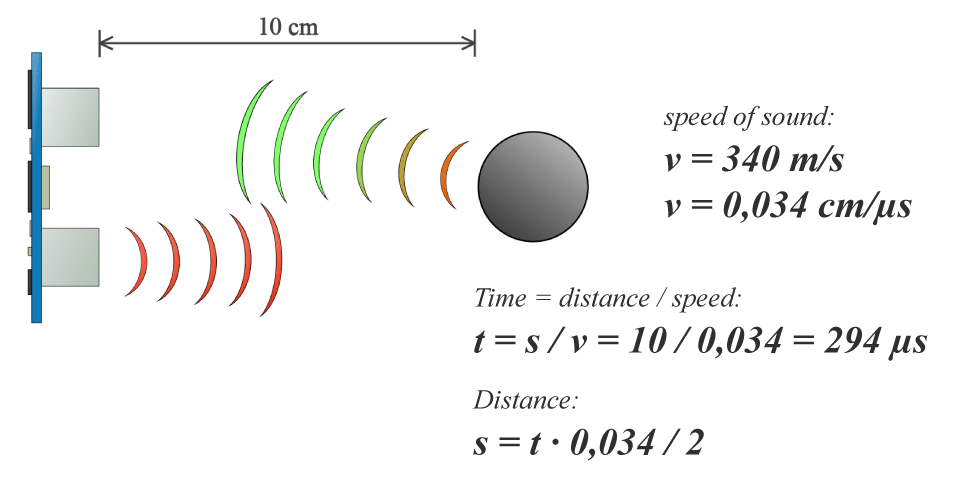
\includegraphics[scale=0.4]{../8-UltraSound/Ultrasonic-Sensor-Equasions.png}
\end{center}

Se configuro al IC en modo monoestable.
\begin{center}
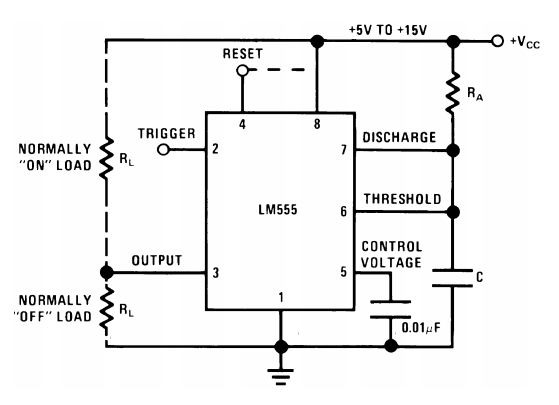
\includegraphics[scale=0.4]{../8-UltraSound/MONO555.png}
\end{center}

Este circuito integrado es desestabilizado cuando recibe un flanco negativo en su pin de \emph{trigger}.
El dispositivo sera accionado mediante un pulsador operado de forma manual. Se utilizo un circuito diferenciador para poder asistir en la generación de flanco descendentes.
\begin{center}
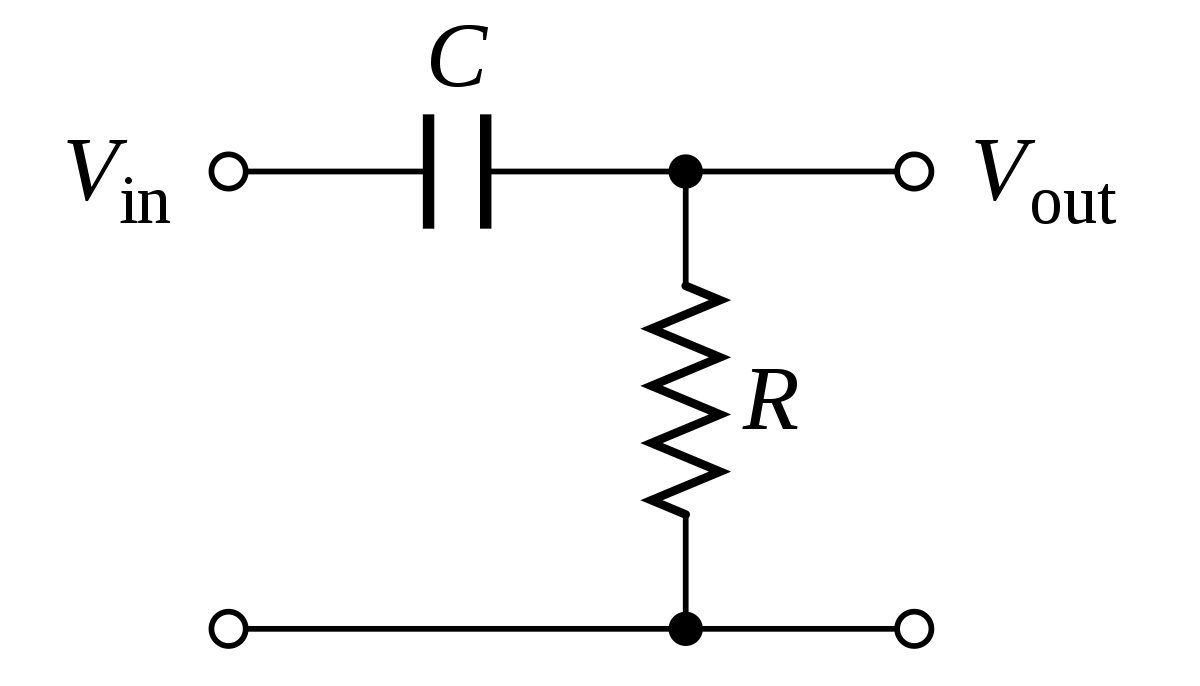
\includegraphics[scale=0.1]{../8-UltraSound/diff.png}
\end{center}

Este pulso luego debera ser negado para poder disparar correctamente al HC-SR04  con el mismo y que cumpla con su  accionar. Por otro lado este pulso es aprovechado para poder dar aviso al sistema que una nueva medición comenzara inminentemente y deben de regresar sus estados a apagado o cero según corresponda. En la sección siguiente se comprendera el porque de la importancia de esta decisión que simplifica mucho la logica del circuito al utilizar menos pasos intermedios.

\section{Contando el tiempo}
Para poder contar el tiempo que tarda el ECHO de rebote es necesario contar con una unidad de referencia a partir de la cual medir el tiempo. Esto lleva a la necesidad de contar con un \emph{clock}
\subsection{Modo Astable LM555}
Para poder generar el clock deseado se empleo otro IC LM555
en configuración astable.
\begin{center}
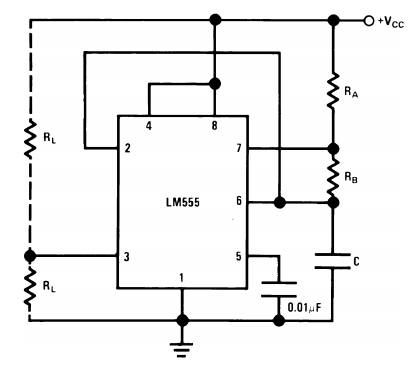
\includegraphics[scale=0.4]{../8-UltraSound/ASTA555.png}
\end{center}

Los componentes fueron elegidos de tal manera que su ciclo de clock fuese lo más cercano a los 100 $\mu S$. El porque se hace evidente viendo la siguiente imagen tomada en el osciloscopio

\begin{center}
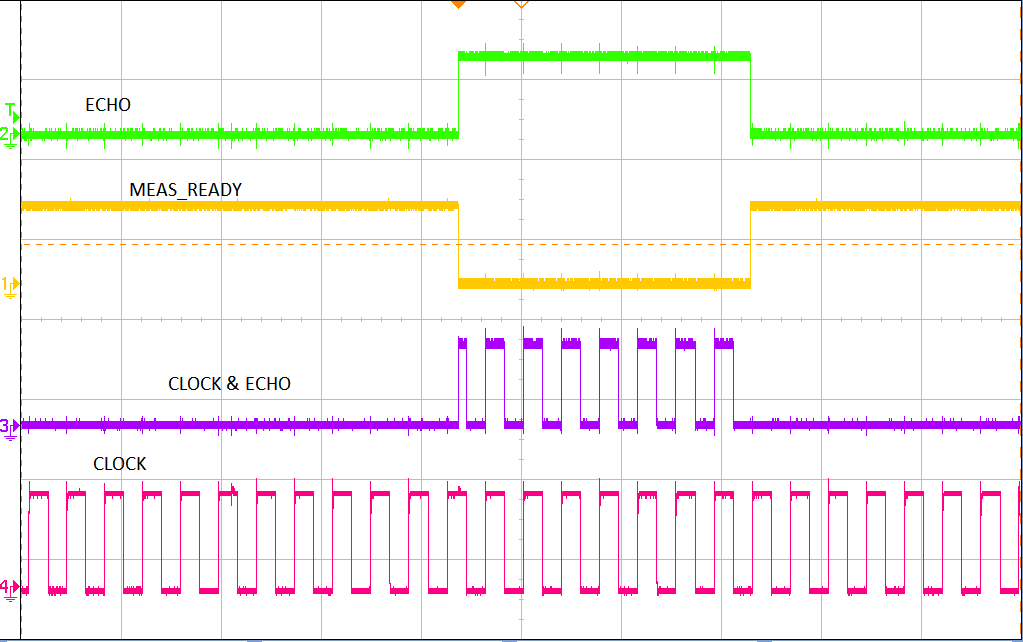
\includegraphics[scale=0.6]{../8-UltraSound/4SLabel.png}
\end{center}

Como se puede apreciar la medida en verde representa el \emph{Echo} recepcionado por el sensor.
La señal en la parte inferior de la imagen representa el clock generado. Por ultimo, la tercera señal representa un \emph{AND} entre el \emph{clock} y el pulso de \emph{Echo} recibido. La señal de color amarillo sera explicada en breve. 
La razón de esta decisión radica en el hecho que el contador elegido adiciona \emph{1} cada vez que ve un flanco negativo
Utilizando un contador binario \emph{CD 4040}. Entonces, al contar (de manera aproximada) la cantidad de periodo de \emph{clock} que entran dentro del ancho del pulso de \emph{Echo}. Luego es posible ver la suma realizada por el contador mediante algún tipo de indicador. En nuestro LED'S. 
Por último tenemos la señal de Measure Ready, esta señal se encarga de avisar al usuario cuando una medida se ha completado. Basicamente este indicador esta apago durante la duración completa del \emph{Echo} y se enciende cuando este finaliza.
\section{Implementacion en PCB}
Esquematico del circuito
\begin{center}
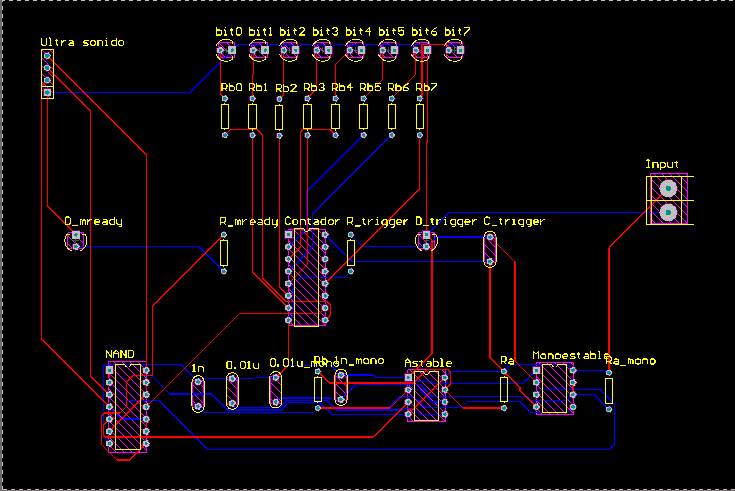
\includegraphics[scale=0.6]{../8-UltraSound/pcb.png}
\end{center}

\section{Retriggering}
Por una cuestión de diseño y de optimización de recursos se decidio no implementar el sistema de bloque de Trigger. Los motivos de dicha decisión fueron los siguientes. En primer lugar, la medición toma un tiempo bastante menor al de la posible reacción de rebote del pulsador. Esto fue testeado al disparar el circuito a frecuencias mayores a 1Khz. Esto nos da la seguridad de que no sera posible por un humano disparar la medición de tal forma de afectarla dado que esta ya se habria realizado. De esta forma es posible ahorrar el costo de utilizar hasta 2 circuitos integrados más dependiendo de como se implemente el sistema de bloqueo.





